
%% milestone.tex
%% V1.0
%% 2014/02/13
%% by Christian Elder
%% This is a file describing the milestone achievements for CS231a project.

%%*************************************************************************
%% Legal Notice:
%% This code is offered as-is without any warranty either expressed or
%% implied; without even the implied warranty of MERCHANTABILITY or
%% FITNESS FOR A PARTICULAR PURPOSE! 
%% User assumes all risk.
%% In no event shall IEEE or any contributor to this code be liable for
%% any damages or losses, including, but not limited to, incidental,
%% consequential, or any other damages, resulting from the use or misuse
%% of any information contained here.
%%
%% All comments are the opinions of their respective authors and are not
%% necessarily endorsed by the IEEE.
%%
%% This work is distributed under the LaTeX Project Public License (LPPL)
%% ( http://www.latex-project.org/ ) version 1.3, and may be freely used,
%% distributed and modified. A copy of the LPPL, version 1.3, is included
%% in the base LaTeX documentation of all distributions of LaTeX released
%% 2003/12/01 or later.
%% Retain all contribution notices and credits.
%% ** Modified files should be clearly indicated as such, including  **
%% ** renaming them and changing author support contact information. **
%%
%% File list of work: IEEEtran.cls, IEEEtran_HOWTO.pdf, bare_adv.tex,
%%                    bare_conf.tex, bare_jrnl.tex, bare_jrnl_compsoc.tex
%%*************************************************************************

% Note that the a4paper option is mainly intended so that authors in
% countries using A4 can easily print to A4 and see how their papers will
% look in print - the typesetting of the document will not typically be
% affected with changes in paper size (but the bottom and side margins will).
% Use the testflow package mentioned above to verify correct handling of
% both paper sizes by the user's LaTeX system.
%
% Also note that the "draftcls" or "draftclsnofoot", not "draft", option
% should be used if it is desired that the figures are to be displayed in
% draft mode.
%
\documentclass[journal]{IEEEtran}
%
% If IEEEtran.cls has not been installed into the LaTeX system files,
% manually specify the path to it like:
% \documentclass[journal]{../sty/IEEEtran}





% Some very useful LaTeX packages include:
% (uncomment the ones you want to load)


% *** MISC UTILITY PACKAGES ***
%
%\usepackage{ifpdf}
% Heiko Oberdiek's ifpdf.sty is very useful if you need conditional
% compilation based on whether the output is pdf or dvi.
% usage:
% \ifpdf
%   % pdf code
% \else
%   % dvi code
% \fi
% The latest version of ifpdf.sty can be obtained from:
% http://www.ctan.org/tex-archive/macros/latex/contrib/oberdiek/
% Also, note that IEEEtran.cls V1.7 and later provides a builtin
% \ifCLASSINFOpdf conditional that works the same way.
% When switching from latex to pdflatex and vice-versa, the compiler may
% have to be run twice to clear warning/error messages.






% *** CITATION PACKAGES ***
%
%\usepackage{cite}
% cite.sty was written by Donald Arseneau
% V1.6 and later of IEEEtran pre-defines the format of the cite.sty package
% \cite{} output to follow that of IEEE. Loading the cite package will
% result in citation numbers being automatically sorted and properly
% "compressed/ranged". e.g., [1], [9], [2], [7], [5], [6] without using
% cite.sty will become [1], [2], [5]--[7], [9] using cite.sty. cite.sty's
% \cite will automatically add leading space, if needed. Use cite.sty's
% noadjust option (cite.sty V3.8 and later) if you want to turn this off.
% cite.sty is already installed on most LaTeX systems. Be sure and use
% version 4.0 (2003-05-27) and later if using hyperref.sty. cite.sty does
% not currently provide for hyperlinked citations.
% The latest version can be obtained at:
% http://www.ctan.org/tex-archive/macros/latex/contrib/cite/
% The documentation is contained in the cite.sty file itself.






% *** GRAPHICS RELATED PACKAGES ***
%
\ifCLASSINFOpdf
   \usepackage[pdftex]{graphicx}
  % declare the path(s) where your graphic files are
  % \graphicspath{{../pdf/}{../jpeg/}}
  % and their extensions so you won't have to specify these with
  % every instance of \includegraphics
  % \DeclareGraphicsExtensions{.pdf,.jpeg,.png}
\else
  % or other class option (dvipsone, dvipdf, if not using dvips). graphicx
  % will default to the driver specified in the system graphics.cfg if no
  % driver is specified.
   \usepackage[dvips]{graphicx}
  % declare the path(s) where your graphic files are
  % \graphicspath{{../eps/}}
  % and their extensions so you won't have to specify these with
  % every instance of \includegraphics
  % \DeclareGraphicsExtensions{.eps}
\fi
% graphicx was written by David Carlisle and Sebastian Rahtz. It is
% required if you want graphics, photos, etc. graphicx.sty is already
% installed on most LaTeX systems. The latest version and documentation can
% be obtained at: 
% http://www.ctan.org/tex-archive/macros/latex/required/graphics/
% Another good source of documentation is "Using Imported Graphics in
% LaTeX2e" by Keith Reckdahl which can be found as epslatex.ps or
% epslatex.pdf at: http://www.ctan.org/tex-archive/info/
%
% latex, and pdflatex in dvi mode, support graphics in encapsulated
% postscript (.eps) format. pdflatex in pdf mode supports graphics
% in .pdf, .jpeg, .png and .mps (metapost) formats. Users should ensure
% that all non-photo figures use a vector format (.eps, .pdf, .mps) and
% not a bitmapped formats (.jpeg, .png). IEEE frowns on bitmapped formats
% which can result in "jaggedy"/blurry rendering of lines and letters as
% well as large increases in file sizes.
%
% You can find documentation about the pdfTeX application at:
% http://www.tug.org/applications/pdftex





% *** MATH PACKAGES ***
%
%\usepackage[cmex10]{amsmath}
% A popular package from the American Mathematical Society that provides
% many useful and powerful commands for dealing with mathematics. If using
% it, be sure to load this package with the cmex10 option to ensure that
% only type 1 fonts will utilized at all point sizes. Without this option,
% it is possible that some math symbols, particularly those within
% footnotes, will be rendered in bitmap form which will result in a
% document that can not be IEEE Xplore compliant!
%
% Also, note that the amsmath package sets \interdisplaylinepenalty to 10000
% thus preventing page breaks from occurring within multiline equations. Use:
%\interdisplaylinepenalty=2500
% after loading amsmath to restore such page breaks as IEEEtran.cls normally
% does. amsmath.sty is already installed on most LaTeX systems. The latest
% version and documentation can be obtained at:
% http://www.ctan.org/tex-archive/macros/latex/required/amslatex/math/





% *** SPECIALIZED LIST PACKAGES ***
%
%\usepackage{algorithmic}
% algorithmic.sty was written by Peter Williams and Rogerio Brito.
% This package provides an algorithmic environment fo describing algorithms.
% You can use the algorithmic environment in-text or within a figure
% environment to provide for a floating algorithm. Do NOT use the algorithm
% floating environment provided by algorithm.sty (by the same authors) or
% algorithm2e.sty (by Christophe Fiorio) as IEEE does not use dedicated
% algorithm float types and packages that provide these will not provide
% correct IEEE style captions. The latest version and documentation of
% algorithmic.sty can be obtained at:
% http://www.ctan.org/tex-archive/macros/latex/contrib/algorithms/
% There is also a support site at:
% http://algorithms.berlios.de/index.html
% Also of interest may be the (relatively newer and more customizable)
% algorithmicx.sty package by Szasz Janos:
% http://www.ctan.org/tex-archive/macros/latex/contrib/algorithmicx/




% *** ALIGNMENT PACKAGES ***
%
%\usepackage{array}
% Frank Mittelbach's and David Carlisle's array.sty patches and improves
% the standard LaTeX2e array and tabular environments to provide better
% appearance and additional user controls. As the default LaTeX2e table
% generation code is lacking to the point of almost being broken with
% respect to the quality of the end results, all users are strongly
% advised to use an enhanced (at the very least that provided by array.sty)
% set of table tools. array.sty is already installed on most systems. The
% latest version and documentation can be obtained at:
% http://www.ctan.org/tex-archive/macros/latex/required/tools/


%\usepackage{mdwmath}
%\usepackage{mdwtab}
% Also highly recommended is Mark Wooding's extremely powerful MDW tools,
% especially mdwmath.sty and mdwtab.sty which are used to format equations
% and tables, respectively. The MDWtools set is already installed on most
% LaTeX systems. The lastest version and documentation is available at:
% http://www.ctan.org/tex-archive/macros/latex/contrib/mdwtools/


% IEEEtran contains the IEEEeqnarray family of commands that can be used to
% generate multiline equations as well as matrices, tables, etc., of high
% quality.


%\usepackage{eqparbox}
% Also of notable interest is Scott Pakin's eqparbox package for creating
% (automatically sized) equal width boxes - aka "natural width parboxes".
% Available at:
% http://www.ctan.org/tex-archive/macros/latex/contrib/eqparbox/





% *** SUBFIGURE PACKAGES ***
%\usepackage[tight,footnotesize]{subfigure}
% subfigure.sty was written by Steven Douglas Cochran. This package makes it
% easy to put subfigures in your figures. e.g., "Figure 1a and 1b". For IEEE
% work, it is a good idea to load it with the tight package option to reduce
% the amount of white space around the subfigures. subfigure.sty is already
% installed on most LaTeX systems. The latest version and documentation can
% be obtained at:
% http://www.ctan.org/tex-archive/obsolete/macros/latex/contrib/subfigure/
% subfigure.sty has been superceeded by subfig.sty.



%\usepackage[caption=false]{caption}
%\usepackage[font=footnotesize]{subfig}
% subfig.sty, also written by Steven Douglas Cochran, is the modern
% replacement for subfigure.sty. However, subfig.sty requires and
% automatically loads Axel Sommerfeldt's caption.sty which will override
% IEEEtran.cls handling of captions and this will result in nonIEEE style
% figure/table captions. To prevent this problem, be sure and preload
% caption.sty with its "caption=false" package option. This is will preserve
% IEEEtran.cls handing of captions. Version 1.3 (2005/06/28) and later 
% (recommended due to many improvements over 1.2) of subfig.sty supports
% the caption=false option directly:
%\usepackage[caption=false,font=footnotesize]{subfig}
%
% The latest version and documentation can be obtained at:
% http://www.ctan.org/tex-archive/macros/latex/contrib/subfig/
% The latest version and documentation of caption.sty can be obtained at:
% http://www.ctan.org/tex-archive/macros/latex/contrib/caption/




% *** FLOAT PACKAGES ***
%
%\usepackage{fixltx2e}
\usepackage{float}
\restylefloat{table}
% fixltx2e, the successor to the earlier fix2col.sty, was written by
% Frank Mittelbach and David Carlisle. This package corrects a few problems
% in the LaTeX2e kernel, the most notable of which is that in current
% LaTeX2e releases, the ordering of single and double column floats is not
% guaranteed to be preserved. Thus, an unpatched LaTeX2e can allow a
% single column figure to be placed prior to an earlier double column
% figure. The latest version and documentation can be found at:
% http://www.ctan.org/tex-archive/macros/latex/base/



%\usepackage{stfloats}
% stfloats.sty was written by Sigitas Tolusis. This package gives LaTeX2e
% the ability to do double column floats at the bottom of the page as well
% as the top. (e.g., "\begin{figure*}[!b]" is not normally possible in
% LaTeX2e). It also provides a command:
%\fnbelowfloat
% to enable the placement of footnotes below bottom floats (the standard
% LaTeX2e kernel puts them above bottom floats). This is an invasive package
% which rewrites many portions of the LaTeX2e float routines. It may not work
% with other packages that modify the LaTeX2e float routines. The latest
% version and documentation can be obtained at:
% http://www.ctan.org/tex-archive/macros/latex/contrib/sttools/
% Documentation is contained in the stfloats.sty comments as well as in the
% presfull.pdf file. Do not use the stfloats baselinefloat ability as IEEE
% does not allow \baselineskip to stretch. Authors submitting work to the
% IEEE should note that IEEE rarely uses double column equations and
% that authors should try to avoid such use. Do not be tempted to use the
% cuted.sty or midfloat.sty packages (also by Sigitas Tolusis) as IEEE does
% not format its papers in such ways.


%\ifCLASSOPTIONcaptionsoff
%  \usepackage[nomarkers]{endfloat}
% \let\MYoriglatexcaption\caption
% \renewcommand{\caption}[2][\relax]{\MYoriglatexcaption[#2]{#2}}
%\fi
% endfloat.sty was written by James Darrell McCauley and Jeff Goldberg.
% This package may be useful when used in conjunction with IEEEtran.cls'
% captionsoff option. Some IEEE journals/societies require that submissions
% have lists of figures/tables at the end of the paper and that
% figures/tables without any captions are placed on a page by themselves at
% the end of the document. If needed, the draftcls IEEEtran class option or
% \CLASSINPUTbaselinestretch interface can be used to increase the line
% spacing as well. Be sure and use the nomarkers option of endfloat to
% prevent endfloat from "marking" where the figures would have been placed
% in the text. The two hack lines of code above are a slight modification of
% that suggested by in the endfloat docs (section 8.3.1) to ensure that
% the full captions always appear in the list of figures/tables - even if
% the user used the short optional argument of \caption[]{}.
% IEEE papers do not typically make use of \caption[]'s optional argument,
% so this should not be an issue. A similar trick can be used to disable
% captions of packages such as subfig.sty that lack options to turn off
% the subcaptions:
% For subfig.sty:
% \let\MYorigsubfloat\subfloat
% \renewcommand{\subfloat}[2][\relax]{\MYorigsubfloat[]{#2}}
% For subfigure.sty:
% \let\MYorigsubfigure\subfigure
% \renewcommand{\subfigure}[2][\relax]{\MYorigsubfigure[]{#2}}
% However, the above trick will not work if both optional arguments of
% the \subfloat/subfig command are used. Furthermore, there needs to be a
% description of each subfigure *somewhere* and endfloat does not add
% subfigure captions to its list of figures. Thus, the best approach is to
% avoid the use of subfigure captions (many IEEE journals avoid them anyway)
% and instead reference/explain all the subfigures within the main caption.
% The latest version of endfloat.sty and its documentation can obtained at:
% http://www.ctan.org/tex-archive/macros/latex/contrib/endfloat/
%
% The IEEEtran \ifCLASSOPTIONcaptionsoff conditional can also be used
% later in the document, say, to conditionally put the References on a 
% page by themselves.





% *** PDF, URL AND HYPERLINK PACKAGES ***
%
%\usepackage{url}
% url.sty was written by Donald Arseneau. It provides better support for
% handling and breaking URLs. url.sty is already installed on most LaTeX
% systems. The latest version can be obtained at:
% http://www.ctan.org/tex-archive/macros/latex/contrib/misc/
% Read the url.sty source comments for usage information. Basically,
% \url{my_url_here}.





% *** Do not adjust lengths that control margins, column widths, etc. ***
% *** Do not use packages that alter fonts (such as pslatex).         ***
% There should be no need to do such things with IEEEtran.cls V1.6 and later.
% (Unless specifically asked to do so by the journal or conference you plan
% to submit to, of course. )


% correct bad hyphenation here
\hyphenation{op-tical net-works semi-conduc-tor}


\begin{document}
%
% paper title
% can use linebreaks \\ within to get better formatting as desired
\title{Milestone: Automatic Camera Network Topology Recognition}
%
%
% author names and IEEE memberships
% note positions of commas and nonbreaking spaces ( ~ ) LaTeX will not break
% a structure at a ~ so this keeps an author's name from being broken across
% two lines.
% use \thanks{} to gain access to the first footnote area
% a separate \thanks must be used for each paragraph as LaTeX2e's \thanks
% was not built to handle multiple paragraphs
%

\author{Christian~Elder,
	     Judson~Wilson,
	     Tony~Vivoli\\
	     Mentor: Alexandre Alahi}

% The paper headers
%\markboth{Journal of \LaTeX\ Class Files,~Vol.~6, No.~1, January~2007}%
%{Shell \MakeLowercase{\textit{et al.}}: Bare Demo of IEEEtran.cls for Journals}
% The only time the second header will appear is for the odd numbered pages
% after the title page when using the twoside option.
% 
% *** Note that you probably will NOT want to include the author's ***
% *** name in the headers of peer review papers.                   ***
% You can use \ifCLASSOPTIONpeerreview for conditional compilation here if
% you desire.


% make the title area
\maketitle

%\begin{abstract}
%%\boldmath
%The abstract goes here.
%\end{abstract}
%% IEEEtran.cls defaults to using nonbold math in the Abstract.
%% This preserves the distinction between vectors and scalars. However,
%% if the journal you are submitting to favors bold math in the abstract,
%% then you can use LaTeX's standard command \boldmath at the very start
%% of the abstract to achieve this. Many IEEE journals frown on math
%% in the abstract anyway.
%
%% Note that keywords are not normally used for peerreview papers.
%\begin{IEEEkeywords}
%Network topology, tracking.
%\end{IEEEkeywords}






% For peer review papers, you can put extra information on the cover
% page as needed:
% \ifCLASSOPTIONpeerreview
% \begin{center} \bfseries EDICS Category: 3-BBND \end{center}
% \fi
%
% For peerreview papers, this IEEEtran command inserts a page break and
% creates the second title. It will be ignored for other modes.
\IEEEpeerreviewmaketitle


% INTRODUCTION
\section{Introduction}
	\indent As the price of digital cameras has dropped, systems of networked cameras have become more prevalent. Furthermore, the cost of computation has dropped low enough that video processing is a viable option for many applications of camera networks. Such applications include analysis of consumer patterns in marketplaces, or use in crime prevention. \\
	\indent While the hardware is now mature and available on the market, there are still many problems to solve and areas for improvement. Manual calibration of such systems still remains an exhausting and expensive task. Cameras that are precalibrated and RGB-D (color and depth) equipped will soon be the norm, but this only solves half of the problem. To make real use of a network of cameras, the position and orientation of each cameras in the world must be known, at least relative to a common frame of reference. Traditionally this requires many many hours of manual work, and does not scale well as more and more cameras are added. \\
	\indent In theory, this calibration information can be inferred from the spatial and temporal information of the scene. Existing techniques can be applied to identify moving objects within the scene from RGB-D data. In the course of this project, we endeavour to create an algorithm which will use the estimated trajectories, or “tracklets” of the objects in the scene, combined with statistical inference techniques and geometry, to estimate the relative locations and orientations of the cameras from which the data originated.



% RELATED WORK
\section{Related Work}
	\indent The problem of determining relationship between cameras with non-overlapping views is not new, and there are several approaches to the problem. Other work has been done to determining the network topology of the camera system \cite{ellis2003,makris2004}. These algorithms typically estimate connectivity between cameras, in the sense of estimating transition probabilities of objects traversing a network and are observed at the camera nodes. They give little insight into the geometric relationship between the cameras. However, these network topologies may be useful in determining corresponding objects between cameras. \\
	\indent \cite{rahimi2004} gives an algorithm to determine the relative position and rotation of cameras within a network, however it requires that a single object move through the network during a manual calibration phase. One of the goals of our algorithm is that it will be able to be calibrated with normal daily traffic in the system, and not require any manual calibration at all. \\
	\indent To our knowledge, no paper has been published which thoroughly outlines an algorithm which can estimate the external calibration of a network of cameras without prior information or manual calibration steps.
	
% ALGORITHM DESCRIPTION
\section{Algorithm}
	\subsection{Algorithm Hypothesis}
		\indent The underlying idea behind the algorithm is that, for the planar world case, relative camera orientations can be determined by identifying the image of a line in both cameras, which constrains the relative positions of two cameras to a line parallel to the imaged line. The position of the camera on this line is then further constrained to a point by identifying a point correspondence on the line image. \\
		\indent While there are many ways that such a line and point could be identified; we chose to use the paths of moving objects. If an object is moving at constant speed and direction, the path will be a perfect line. If the object produces a linear tracklet in the first camera, then a speed and direction estimate can be determined. Afterwards, any observation by any camera at a later time can be extrapolated to calculate a corresponce to a specific point on this line in the first camera’s coordinate system. If a second camera observes this object, a point correspondence and a line correspondence will be known. This is enough information to determine the relative position and angles of the two cameras in the 2D floorplan. \\
		\indent Given a sufficient number of correspondences between many cameras, the external calibration can be determined. \\
		
% Dataset
\section{Dataset}
	\indent Our dataset comes from a camera system installed in the Lausanne railway station, provided by Alexandre Alahi. The system uses RGB-D cameras to detect moving objects through the station, and a software pipeline is used to create tracklet data which describes the motion of objects through the cameras’ fields of view. The data is given in planar (x,y) coordinates for each timestep, in the coordinate system of the observing camera, as the object moves along a track. Object identity is not tracked between cameras.

% RESULTS
\section{Results}
	\indent We ran our current algorithm on simulated data with varying path curvature and additive Gaussian noise (see Figures~\ref{curvy_paths},\ref{paths}), generating plots of the estimated camera relation for each correspondence (see Figure~\ref{point_cloud}). When we injected no noise or false correspondences, the resulting camera relations mapped to exactly the correct values. As we introduced noise, curved paths, varying velocity, and false correspondences, the resulting estimates became more diffuse. However, the data points are still clustered around the correct values. \\
	\indent Figure~\ref{point_cloud} depicts estimates computed from tracks with little noise and few tracks per time interval, resulting in very dense clusters about the actual relative orientations of the cameras. Figure~\ref{noisy_point_cloud} shows camera relation estimates produced when multiple tracks occur per time interval, resulting in more false correspondences. There is, however, still a distinct cluster around the actual relative orientations of the cameras.

	\begin{figure}
		\centering
		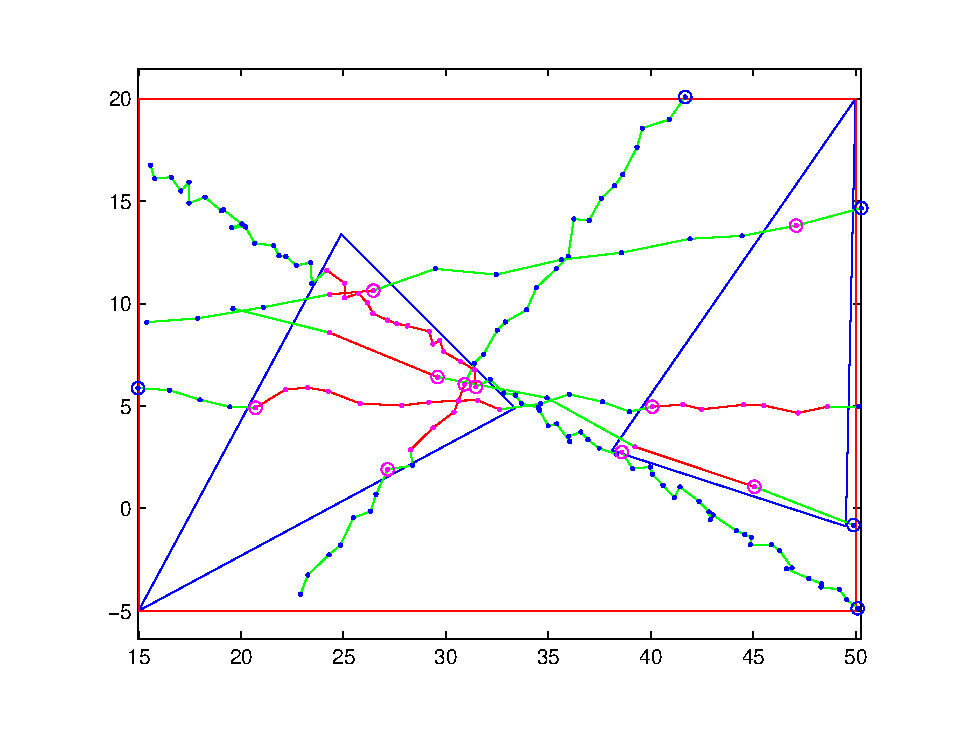
\includegraphics[width=4in]{./curvy_paths.eps}
		\caption{\textbf{Noisy Simulation} Simulation introduces Gaussian noise in both 											speed and direction of movement across the 											world}
		\label{curvy_paths}
	\end{figure}

	\begin{figure}
		\centering
		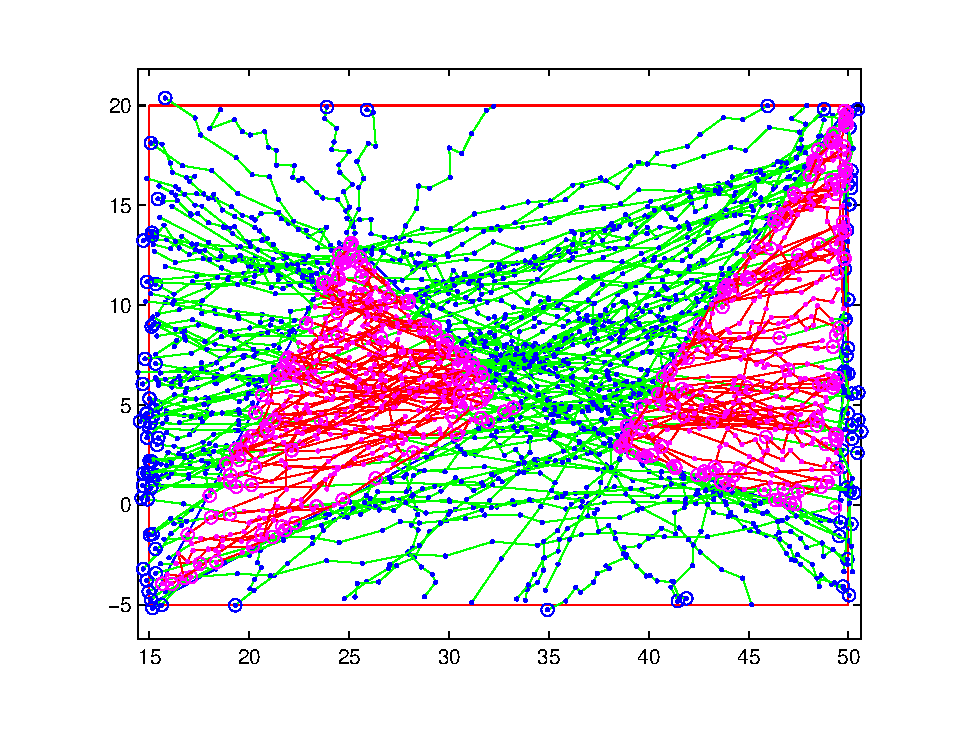
\includegraphics[width=4in]{./paths.eps}
		\caption{\textbf{Simulated Track Map}  Simulation produces tracks across world 
										space (green), which intersect cameras 
										field of view (pink triangle). Data input to
										localization algorithm is shown in pink}
		\label{paths}
	\end{figure}

	\begin{figure}
		\centering
		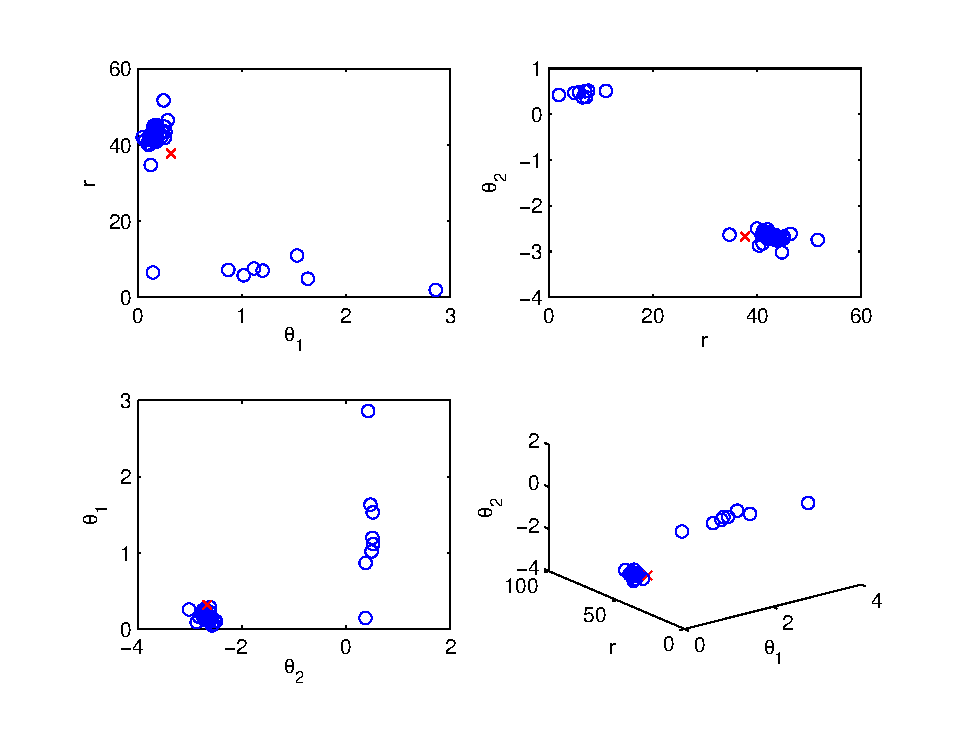
\includegraphics[width=4in]{./point_cloud.eps}
		\caption{\textbf{Estimated Camera Relation} The algorithm produces an estimate 
											of the camera relation between two
											cameras for each correspondence. 
											The above plots show the estimates
											for the camera relation from
											Figure~\ref{paths}.}
		\label{point_cloud}
	\end{figure}

%	\begin{figure}[!t]
%		\centering
%		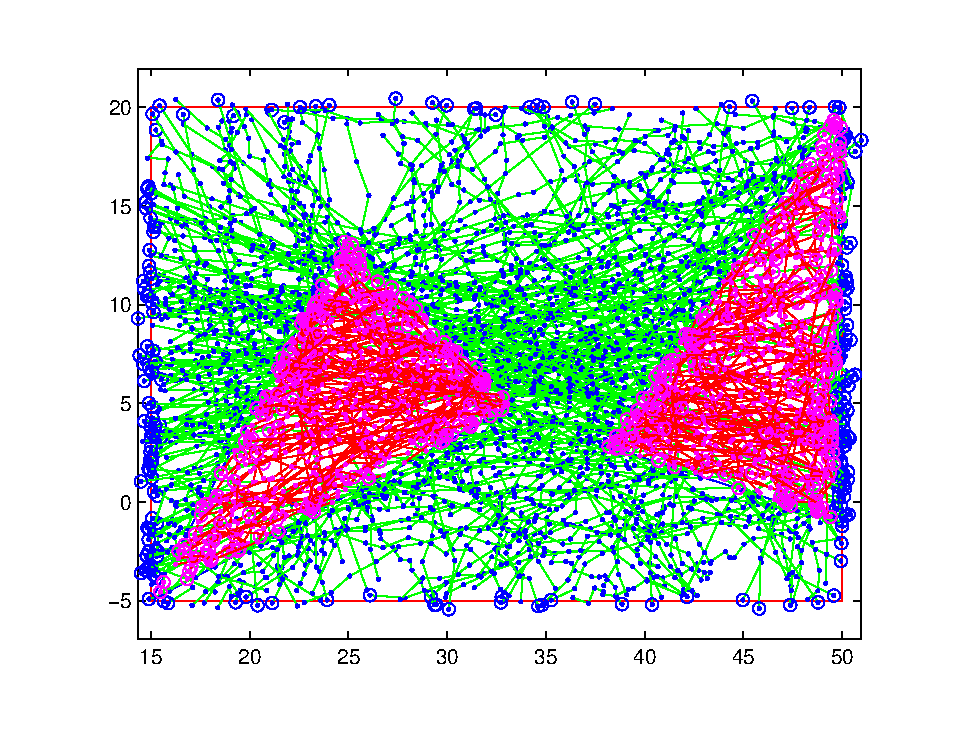
\includegraphics[width=4in]{./noisy_paths.eps}
%		\caption{Noisy Paths}
%		\label{noisy_paths}
%	\end{figure}
	
	\begin{figure}[H]
		\centering
		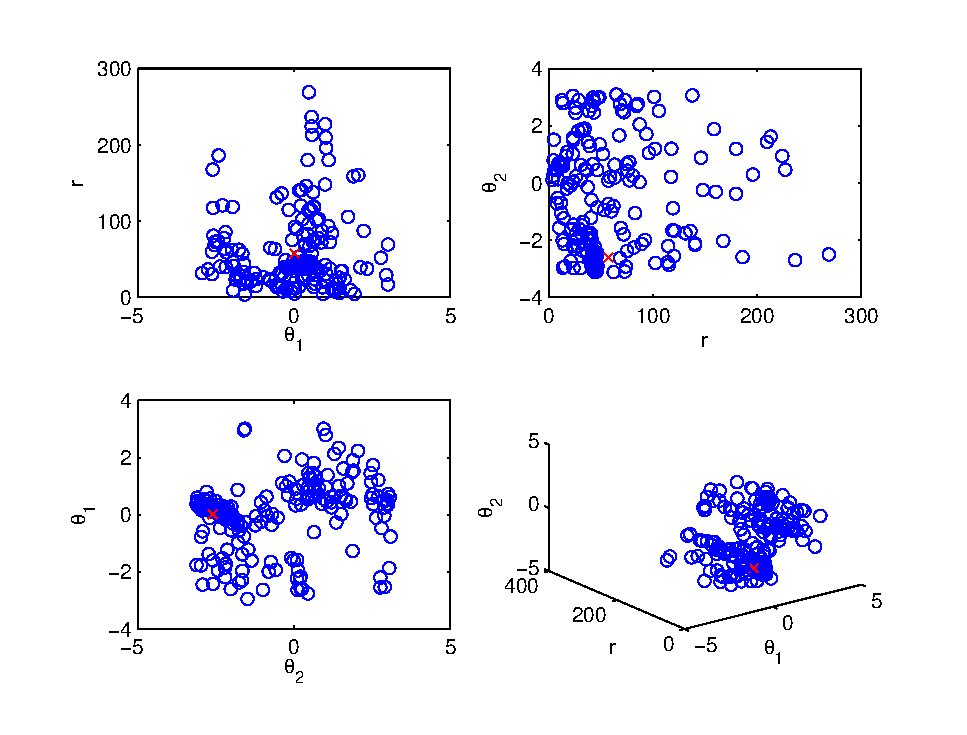
\includegraphics[width=4in]{./noisy_point_cloud.eps}
		\caption{\textbf{Estimated Camera Relation with More False Correspondences} 
					The estimates above are produced from tracks which produce
					more false correspondences due to multiple tracks entering and
					exiting the fields of view at a given timestep.}
		\label{noisy_point_cloud}
	\end{figure}


% MILESTONE GOALS
\section{Milestone Goals}
	See Table I and II for achieved and remaining milestones.
	\begin{table}[H]
		\renewcommand{\arraystretch}{1.3}
		\caption{Milestones Achieved}
		\label{table_example}
		\centering
			\begin{tabular}{l|l}
				\hline
				\bfseries Week & \bfseries Milestone\\
				\hline
				1/26-2/1 & - Determine Project Topic\\
						 & - Write Project Proposal\\
						 & \textbf{Thurs 1/30 - Proposal Due}\\
				\hline
				2/2-2/8 & - Literature Survey\\
					       & - Familiarize with Data Set\\
					       & - Begin Algorithm Dev. - Toy Problem\\
				\hline
				2/9-2/15 & - Finish Toy Problem\\
						 & - Algorithm Dev. - Handpicked Data\\
						 & - Write Milestone Progress Report\\
						 & \textbf{Thurs 2/13 - Milestone Progress Due}\\
				\hline
			\end{tabular}
	\end{table}
	\begin{table}[H]
	\renewcommand{\arraystretch}{1.3}
	\caption{Remaining Milestones}
	\label{table_example_2}
	\centering
		\begin{tabular}{l|l}
			\hline
			\bfseries Week & \bfseries Milestone\\
			\hline
			2/16-2/22 & - Algorithm Dev. - Continue with Handpicked Data\\
					   & - Expand Dataset, Test, Develop\\
			\hline
			2/23-3/1 & - Expand Dataset, Test, Develop\\
			\hline
			3/2-3/8 & - Measure Performance with Fewer Cameras\\
			\hline
			3/9-3/15 & - Produce Graphical Demo of Results\\
					 & \textbf{Tues 3/11 - Project Presentations (I)}\\
					 & \textbf{Tues 3/11 - Project Presentations (I)}\\
			\hline
			3/16-3/19 & - Write Final Report\\
					   & \textbf{Wed 3/19 - Final Report Due}\\
			\hline
		\end{tabular}
	\end{table}
	
\section{Conclusion}
The conclusion goes here.





% if have a single appendix:
%\appendix[Proof of the Zonklar Equations]
% or
%\appendix  % for no appendix heading
% do not use \section anymore after \appendix, only \section*
% is possibly needed

% use appendices with more than one appendix
% then use \section to start each appendix
% you must declare a \section before using any
% \subsection or using \label (\appendices by itself
% starts a section numbered zero.)
%


% Can use something like this to put references on a page
% by themselves when using endfloat and the captionsoff option.
%\ifCLASSOPTIONcaptionsoff
%  \newpage
%\fi



% trigger a \newpage just before the given reference
% number - used to balance the columns on the last page
% adjust value as needed - may need to be readjusted if
% the document is modified later
%\IEEEtriggeratref{8}
% The "triggered" command can be changed if desired:
%\IEEEtriggercmd{\enlargethispage{-5in}}

% references section

% can use a bibliography generated by BibTeX as a .bbl file
% BibTeX documentation can be easily obtained at:
% http://www.ctan.org/tex-archive/biblio/bibtex/contrib/doc/
% The IEEEtran BibTeX style support page is at:
% http://www.michaelshell.org/tex/ieeetran/bibtex/
%\bibliographystyle{IEEEtran}
% argument is your BibTeX string definitions and bibliography database(s)
%\bibliography{IEEEabrv,../bib/paper}
%
% <OR> manually copy in the resultant .bbl file
% set second argument of \begin to the number of references
% (used to reserve space for the reference number labels box)
\begin{thebibliography}{1}

\bibitem{knight2003}
O. Javed, Z. Rasheed, O. Alatas, and M. Shah, \emph{KNIGHT™: a real time surveillance system for multiple and non-overlapping cameras}, in Proceedings of 2003 International Conference on Multimedia and Expo, 2003, pp. I-649.

\bibitem{ellis2003}
T. Ellis, D. Makris, J. Black, \emph{Learning a multi-camera topology}, in Joint IEEE Workshop on Visual Surveillance and Performance Evaluation of Tracking and Surveillance (VS-PETS), 2003, pp. 165-171.

\bibitem{makris2004}
D. Makris, T. Ellis, J. Black, \emph{Bridging the gaps between cameras}, in Proceedings of the 2004 IEEE Computer Society Conference on Computer Vision and Pattern Recognition, 2004, pp. II-205.

\bibitem{rahimi2004}
A. Rahimi, B. Dunagan, and T. Darrell, \emph{Simultaneous calibration and tracking with a network of non-overlapping sensors}, in Proceedings of the 2004 IEEE Computer Society Conference on Computer Vision and Pattern Recognition, 2004, pp. I-187.

\end{thebibliography}

% Can be used to pull up biographies so that the bottom of the last one
% is flush with the other column.
\enlargethispage{-5in}



% that's all folks
\end{document}


